\documentclass[a4paper, 11pt, french]{article}
\usepackage[left=1cm, right=1cm, top=1.5cm, bottom=1.5cm]{geometry}
\usepackage[frenchb]{babel}
\usepackage[T1]{fontenc}
\usepackage{tikz}
\usepackage{xcolor}

\definecolor{mylightblue}{HTML}{6699FF}
\definecolor{myblue}{HTML}{3366CC}
\definecolor{mydarkblue}{HTML}{003399}
\definecolor{mylightgreen}{HTML}{99CC33}
\definecolor{mygreen}{HTML}{00CC00}
\definecolor{mygreenishyellow}{HTML}{669900}
\definecolor{myyellow}{HTML}{FFCC00}
\definecolor{myorange}{HTML}{FF9900}
\definecolor{myred}{HTML}{CC0000}

\pagenumbering{gobble}


\begin{document}
	\section*{Graphe}
	\fontfamily{cmtt}
	\begin{center}
		\resizebox{0.85\columnwidth}{!}{%
			\begin{tikzpicture}[scale=1]
			\tikzset{% This is the style settings for nodes
				lightbluenode/.style={circle,minimum size=1cm,fill=mylightblue!20,draw=mylightblue,line width=0.5mm},
				bluenode/.style={circle,minimum size=1cm,fill=myblue!20,draw=myblue,line width=0.5mm},
				darkbluenode/.style={circle,minimum size=1cm,fill=mydarkblue!20,draw=mydarkblue,line width=0.5mm},
				lightgreennode/.style={circle,minimum size=1cm,fill=mylightgreen!20,draw=mylightgreen,line width=0.5mm},
				greennode/.style={circle,minimum size=1cm,fill=mygreen!20,draw=mygreen,line width=0.5mm},
				greenishyellownode/.style={circle,minimum size=1cm,fill=mygreenishyellow!20,draw=mygreenishyellow,line width=0.5mm},
				yellownode/.style={circle,minimum size=1cm,fill=myyellow!20,draw=myyellow,line width=0.5mm},
				orangenode/.style={circle,minimum size=1cm,fill=myorange!20,draw=myorange,line width=0.5mm},
				rednode/.style={circle,minimum size=1cm,fill=myred!20,draw=myred,line width=0.5mm}}
			\node[lightbluenode] (0) at (0,2) {C1};
			\node[bluenode] (1) at (-2,1) {A1};
			\node[orangenode] (2) at (2,1) {A2};
			\node[darkbluenode] (3) at (0,0) {C2};
			\node[lightgreennode] (4) at (-2,-1) {C3};
			\node[yellownode] (5) at (2,-1) {C4};
			\node[greennode] (6) at (-1,-2.5) {A3};
			\node[greenishyellownode] (7) at (1,-2.5) {A4};
			\node[rednode] (8) at (0,-4) {C5};
	
			\draw[-stealth,very thick](0) to[bend right] (1);
			\draw[-stealth,very thick](2) to[bend right] (0);
			\draw[-stealth,very thick](1) to (3);
			\draw[-stealth,very thick](3) to (2);
			\draw[-stealth,very thick](1) to (4);
			\draw[-stealth,very thick](5) to (2);
			\draw[-stealth,very thick](4) to[bend right] (6);
			\draw[-stealth,very thick](7) to[bend right] (5);
			\draw[-stealth,very thick](6) to (7);
			\draw[-stealth,very thick](6) to[bend right] (8);
			\draw[-stealth,very thick](8) to[bend right] (7);
		\end{tikzpicture}
	}
	\end{center}
	\section*{Schéma}
	\begin{center}
		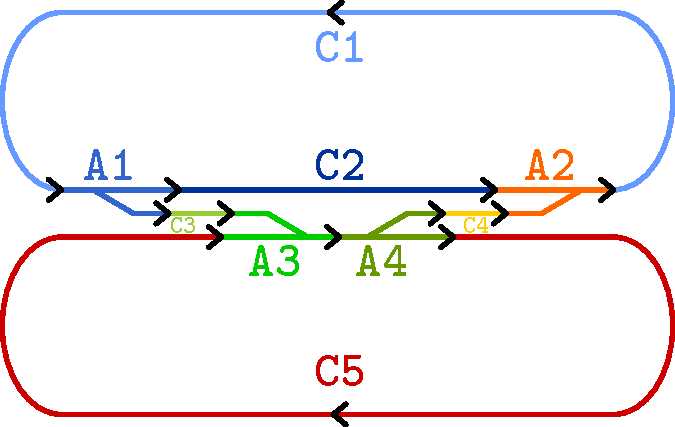
\includegraphics[keepaspectratio,height=12cm]{schema_circuit.pdf}
	\end{center}
\end{document}